Production of high-energy SM particles in a WD will result in heating of the stellar medium.
The critical quantity to understand is the length scale over which such heating occurs---this scale determines the efficiency of the heating event in triggering runaway fusion, as described by condition~\eqref{eq:energy_boom_condition}.
Note that this is a question of purely SM physics.
The unknown physics of DM will serve only to set the initial properties of the SM particles.

We find that SM particles efficiently heat the WD regardless of species or energy (neutrinos are a slight exception)---the heating length is typically less than or of order the trigger size $\lambda_T$.
This is accomplished primarily through hadronic showers initiated by collisions with carbon ions.
In some cases electromagnetic showers are important, however at high energies these are suppressed by density effects and even photons and electrons are dominated by hadronic interactions.
These showers rapidly stop high-energy particles due to their logarithmic nature, transferring the energy into a cloud of low-energy particles which heat the medium through elastic scatters.
A schematic for the flow of energy during deposition is given in Figure~\ref{fig:cooling-cartoon}.
In this light, the WD operates analogously to a particle detector, including hadronic and electromagnetic ``calorimeter'' components.
Runaway fusion provides the necessary amplification to convert a detected event into an observable signal.

\begin{figure*}
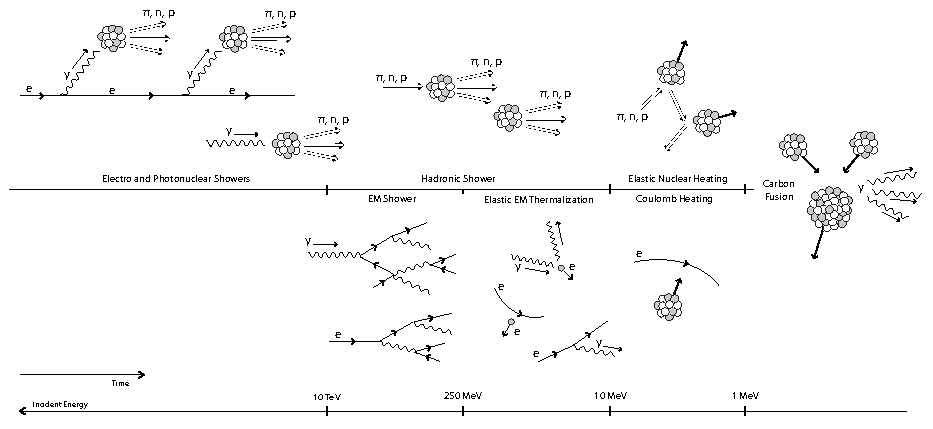
\includegraphics[scale=1.15]{cooling-cartoon.pdf}
\caption{Dominant energy loss and thermalization processes in the WD as a function of energy, with energy decreasing towards the right.
Hadronic processes are shown in the upper panel and EM processes in the lower panel.
High energy particles will induce showers that terminate into elastic thermalization of the WD ions, moving from left to right in the diagram.
The quoted energies are for a $\sim 1.37 ~M_{\astrosun}$ WD, although the cartoon is qualitatively the same for all densities.}
\label{fig:cooling-cartoon}
\end{figure*}


The remainder of this section will discuss the above heating process in more detail.
We summarize the dominant source of energy loss and the resulting stopping lengths $\lambda$ for SM particles of incident kinetic energy $\epsilon$, approximated by
\begin{equation}
\lambda \sim \frac{\epsilon}{dE/dx},
\end{equation}
where $dE/dx$ is the stopping power in the WD medium.
Stopping lengths are plotted in Figures~\ref{fig:SPhighHad} and~\ref{fig:SPhighEM}, and a detailed treatment of the stopping powers is given in Appendix~\ref{sec:wdpdg}.
We will consider incident light hadrons, photons, electrons, and neutrinos---as we are concerned with triggering runaway fusion, we restrict our attention to energies $\epsilon \gg T_f \sim \text{MeV}$.


\subsection{High-Energy Showers}

\paragraph{Hadronic Showers.}
Incident hadrons with kinetic energy larger than the nuclear binding scale $\sim 10~\MeV$ will undergo violent inelastic collisions with carbon ions resulting in an $\OO(1)$ number of secondary hadrons.
This results in a roughly collinear shower of hadrons of size
\begin{align}
\label{eq:hadlength}
  X_\text{had} &\sim \frac{1}{n_\ion \sigma_\text{inel}} \log\l\frac{\epsilon}{10 ~\MeV}\r \\
  &\approx 10^{-6} ~\text{cm}
  \l\frac{10^{32}~\text{cm}^{-3}}{n_\text{ion}}\r. \nonumber
\end{align}
where the inelastic nuclear cross section is $\sigma_\text{inel} \approx 100 ~\text{mb}$ and we have taken the logarithm to be $\sim 10$.
The shower terminates into pions and nucleons of energy $\sim 10~\MeV$, whose cooling is discussed below.
Note that neutral pions of energy $10 - 100 ~\text{MeV}$ have a decay length to photons of $\delta_{\pi^0} \sim 10^{-6} ~\text{cm}$.
Hadronic showers will therefore generate an electromagnetic component carrying an $\OO(1)$ fraction of the energy.

\begin{figure}
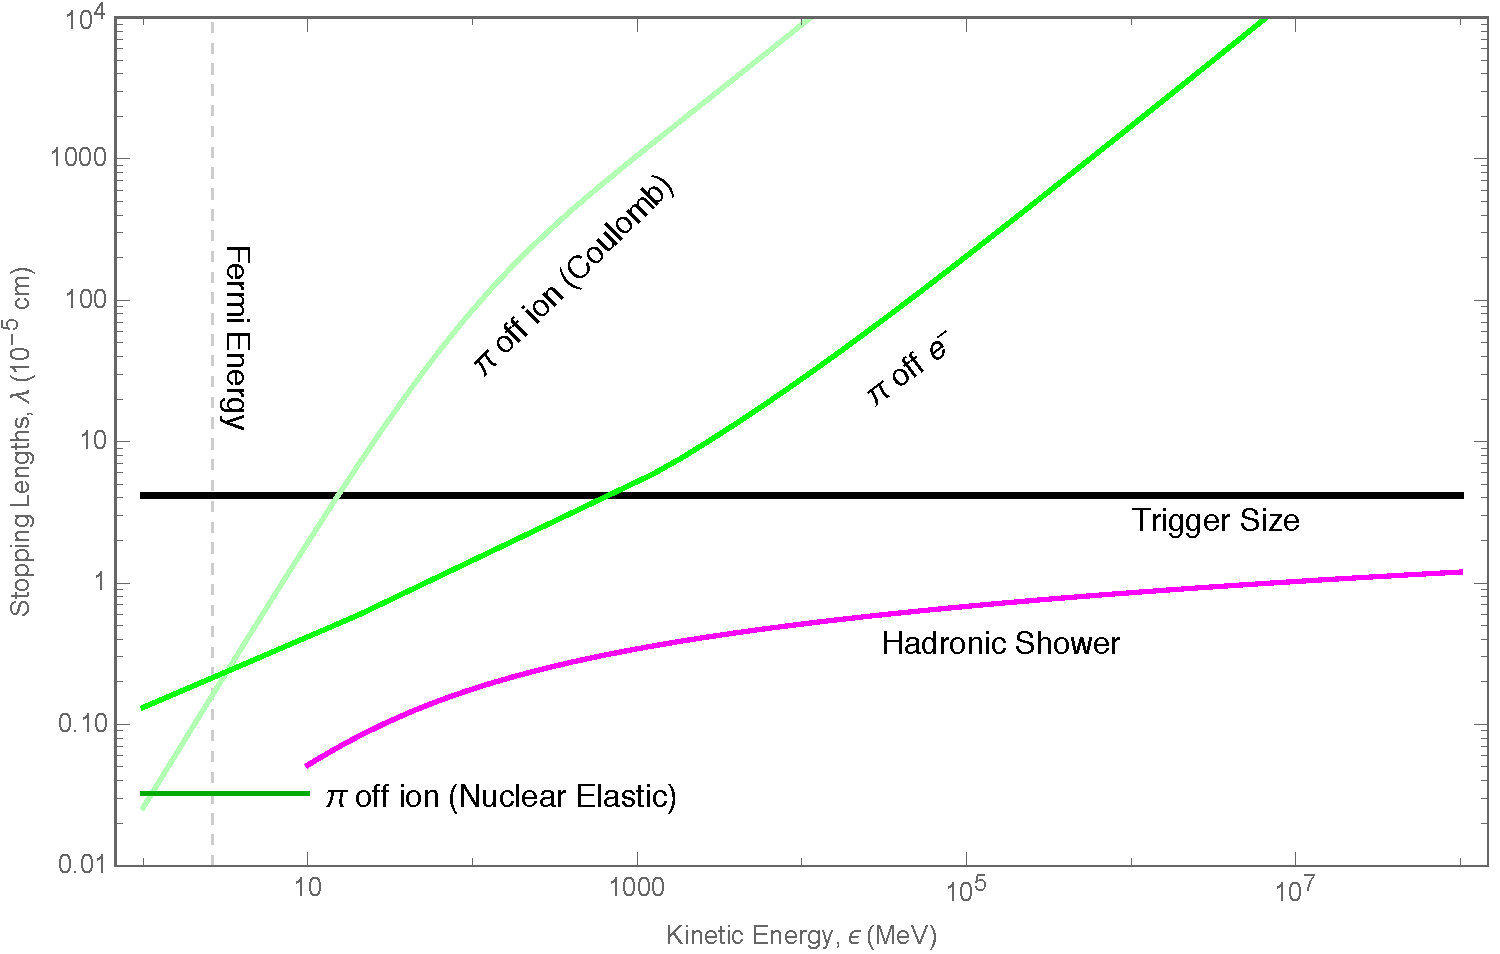
\includegraphics[scale=.3]{SPhighHad.pdf}
\caption{Stopping lengths for incident hadrons as a function of kinetic energy in a WD of density $n_\text{ion} \sim 10^{31}~\text{cm}^{-3}$ ($\approx 1.25 ~M_{\astrosun}$), including the hadronic shower length (magenta).
Any discontinuities in the stopping lengths are due to approximate analytic results in the different energy regimes.
See Appendix~\ref{sec:wdpdg} for calculation details.
}
\label{fig:SPhighHad}
\end{figure}

\begin{figure}
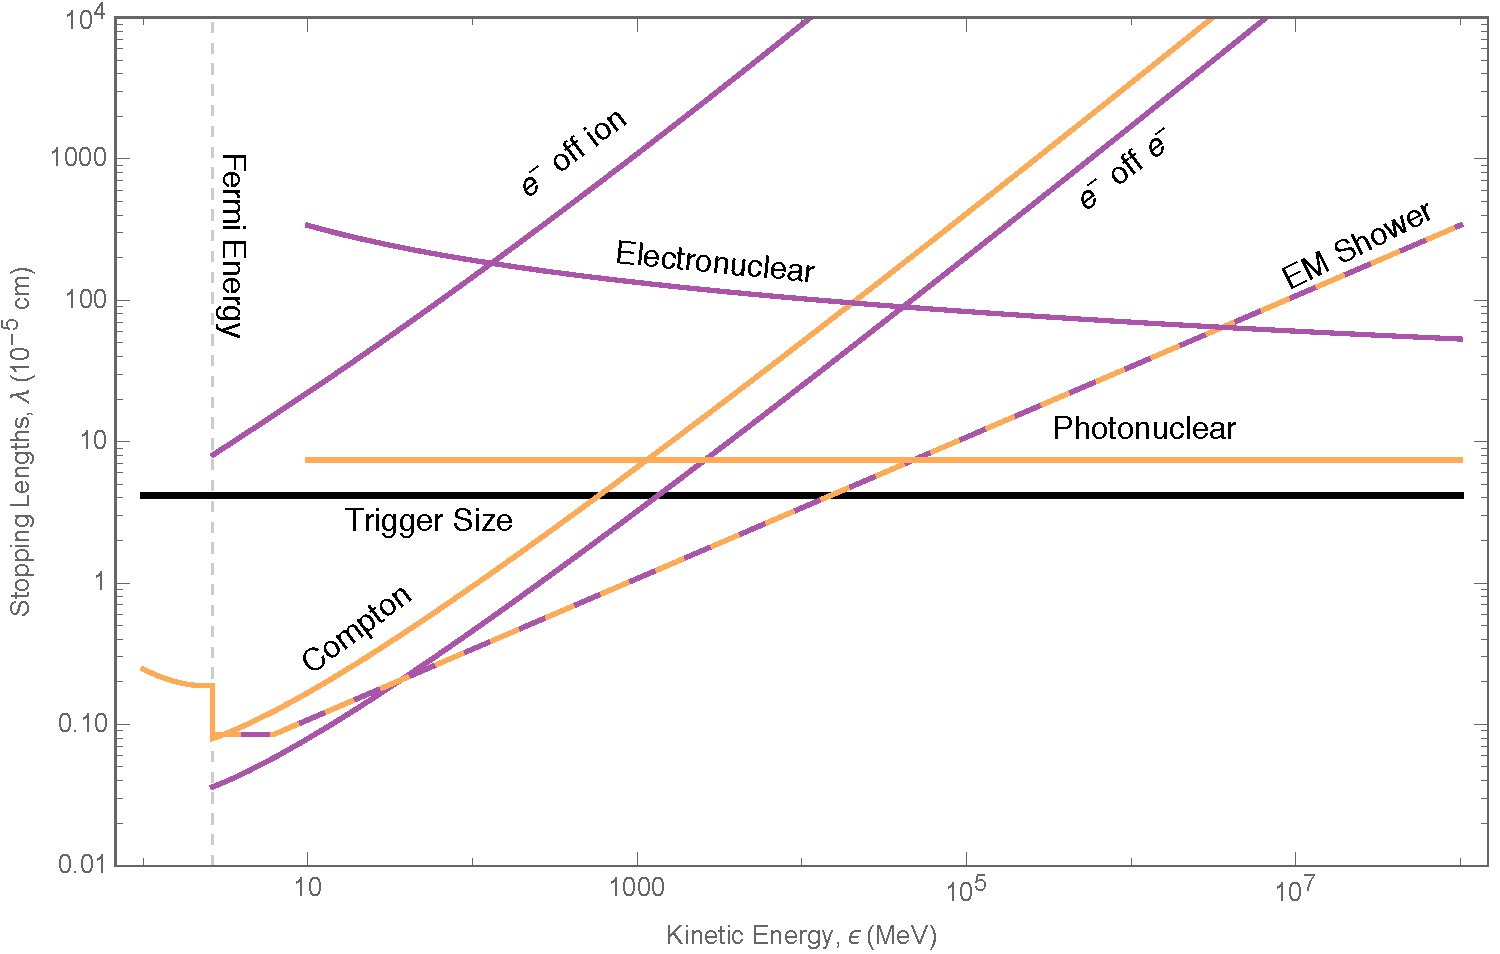
\includegraphics[scale=.3]{SPhighEM.pdf}
\caption{Stopping lengths of incident photons (orange) and electrons (purple) as a function of kinetic energy in a WD of density $n_\text{ion} \sim 10^{31}~\text{cm}^{-3}$ ($\approx 1.25 ~M_{\astrosun}$), including the EM shower length (dashed).
Any discontinuities in the stopping lengths are due to approximate analytic results in the different energy regimes.
See text for details.
}
\label{fig:SPhighEM}
\end{figure}


\paragraph{Photonuclear and Electronuclear Showers.}
A photon or electron can directly induce hadronic showers via production of a quark-antiquark pair, depicted in Figure~\ref{fig:electrophotonuclear-diagram}.
The LPM effect, discussed below, ensures that these process dominate the stopping of photons and electrons at high energies, $\epsilon \gtrsim 10^4-10^6~\GeV$.

\begin{figure}
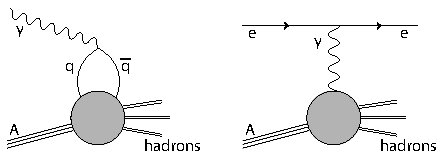
\includegraphics[scale=1.0]{electrophotonuclear-diagram.pdf}
\caption{Photonuclear (left) and Electronuclear (right) interactions. The shaded region contains, at high energies, the familiar point-like processes of deep inelastic scattering and for energies below $\Lambda_\x{QCD}$ is best described by exchange of virtual mesons.}
\label{fig:electrophotonuclear-diagram}
\end{figure}

The only substantial difference between photonuclear showers and purely hadronic ones is that they require a longer distance to initiate.
Roughly, the photonuclear cross section is suppressed relative to the hadronic inelastic cross section $\sigma_\text{inel}$ by a factor of $\alpha$, and so the photon range is
\begin{align}
\label{eq:photonuclength}
  \lambda_{\gamma A} \approx 10^{-5} ~\text{cm} \l\frac{10^{32}~\text{cm}^{-3}}{n_\text{ion}}\r.
\end{align}
Here $\lambda_{\gamma A}$ is the distance to initiate a hadronic shower, whereas the shower itself extends a distance $X_\text{had}$.
Note that $\lambda_{\gamma A}$ is of order the trigger size.

The electronuclear showers are qualitatively different, as the electron survives the interaction.
This process is best described as a continuous energy loss of the electron, due to radiation of virtual photons into hadronic showers.
The stopping power is again radiative, which gives the constant stopping length
\begin{align}
\label{eq:electronuclength}
  \lambda_{eA}
  \approx 10^{-4} ~\text{cm} \l\frac{10^{32}~\text{cm}^{-3}}{n_\text{ion}}\r.
\end{align}
This is suppressed by an additional factor of $\alpha$ relative to the photonuclear interaction, although a full calculation also yields an $\OO(10)$ logarithmic enhancement.
We see that the electronuclear length scale $\lambda_{eA}$ is at most larger than the trigger size by an order of magnitude.

\paragraph{Electromagnetic Showers.}
Of course, electrons and photons can also shower through successive bremsstrahlung and pair-production.
An electromagnetic shower proceeds until a critical energy $\sim 100 ~\MeV$, at which point these radiative processes become subdominant to elastic Coulomb and Compton scattering.
Below this scale radiation can still be important, though electromagnetic showers do not occur.
Note that bremsstrahlung and pair-production are strictly forbidden for incident energies below the Fermi energy $E_F$.

At sufficiently high electron/photon energies and nuclear target densities, electromagnetic showers are elongated due to the ``Landau-Pomeranchuk-Migdal" (LPM) effect.
High-energy radiative processes necessarily involve small momentum transfers to nuclei.
These soft virtual photons cannot be exchanged with only a single ion, but rather interact simultaneously with multiple ions.
This generates a decoherence, suppressing bremsstrahlung/pair-production above an energy $E_\text{LPM}$ which scales inversely with density:
\begin{align}
    E_\text{LPM} \approx 1~\MeV
    \l \frac{10^{32}~\text{cm}^{-3}}{n_\text{ion}} \r
\end{align}
The corresponding shower lengths are
\begin{align}
  X_\text{EM} &\approx X_0 \cdot
  \begin{cases}
  \l \frac{\epsilon}{E_\text{LPM}} \r^{1/2} & \epsilon > E_\text{LPM} \\
  \;\;\;\;\;\, 1 & \epsilon < E_\text{LPM}
  \end{cases}
\end{align}
where
\begin{align}
  X_0 &\approx 10^{-7} ~\text{cm}
  \l\frac{10^{32}~\text{cm}^{-3}}{n_\text{ion}}\r.
\end{align}
is the unsuppressed EM shower length.
See Appendix~\ref{sec:emshowers} for details.
At the highest WD densities radiative processes are always LPM-suppressed, while at lower densities we observe both regimes.
We emphasize that for all densities, throughout the energy range where it is relevant, the length of electromagnetic showers is never parametrically larger than the trigger size.

\paragraph{Neutrinos.}
Neutrinos scatter off nuclei with a cross section that increases with energy.
In these interactions, an $\OO(1)$ fraction of the neutrino energy is transferred to the nucleus with the rest going to produced leptons---this is sufficient to start a hadronic shower \cite{Gandhi:1998ri, Formaggio:2013kya}.
At an energy of $\sim 10^{11} ~\GeV$, \cite{Gandhi:1998ri} calculates the neutrino-nuclear cross section to be $\sim 10^{-32} ~\cm^2$.
Conservatively assuming this value for even higher energies, we find a neutrino mean free path in a WD of order $\sim 10 ~\cm$.
While this distance is much too large to heat a WD via the release of multiple low-energy neutrinos, for a single neutrino it is simply a displacement after which a compact shower of size $X_\text{had}$ occurs.
As such, a \emph{single} high-energy neutrino will heat the star just as high-energy hadrons do.

\subsection{Low-Energy Elastic Heating}
The showers of high-energy particles described above terminate in a cloud of low-energy $\epsilon \sim 10~\MeV$ neutrons, protons, and charged pions, and $\epsilon \sim 10-100~\MeV$ electrons and photons.
Of course, particles at these energies may also be directly produced by the DM.
At these energies, elastic nuclear, Coulomb, and Compton scatters dominate and eventually lead to the thermalization of ions.

\paragraph{Hadrons.}
Neutral hadrons are the simplest species we consider, interacting at low-energies only through elastic nuclear scatters with cross section $\sigma_\text{el} \approx \text{b}$.
Note that the large ion mass requires $\sim 10 - 100$ scatters to transfer the hadron's energy in the form of a random-walk.
This elastic heating range is
\begin{align}
 \lambda_\text{el} &\approx
 10^{-7} ~\text{cm} \l\frac{10^{32}~\text{cm}^{-3}}{n_\text{ion}}\r,
\end{align}
and is always less than the trigger size.

Charged hadrons are also subject to Coulomb interactions, which would provide the dominant stopping in terrestrial detectors.
In this case, however, Coulomb scatters off degenerate WD electrons are strongly suppressed and charged hadrons predominantly undergo elastic nuclear scatters like their neutral brethren.
This suppression is due to (1) motion of the electrons, which fixes the relative velocity to be $\OO(1)$ and removes the enhancement of Coulomb stopping usually seen at low velocity, and (2) Pauli blocking, which forces the incident particle to scatter only electrons near the top of the Fermi sea.
For an incident particle with velocity $v_\x{in} \ll 1$, the first effect suppresses the stopping power by a factor of $v_\x{in}^2$ relative to that off stationary, non-degenerate electrons and the second by an additional factor of $v_\x{in}$.
Note that there is a small range of energies in which Coulomb scatters off ions dominate the stopping of charged hadrons---either way, both length scales are well below the trigger size.

\paragraph{Electrons and Photons.}
For electrons and photons below $\sim 100 ~\MeV$ the dominant interactions are Coulomb scatters off WD electrons and Compton scatters, respectively.
The length scale of these processes is smaller than any interaction with ions, and so these electrons and photons will thermalize into a compact electromagnetic ``gas" with a size set by the radiative length scale $X_\text{EM}$.
The EM gas will cool and diffuse to larger length scales, eventually allowing thermalization with nuclei via the subdominant Coulomb scatters of electrons off ions. 
The photons of the EM gas will not undergo photonuclear showers here, as the gas will cool below $\sim 10~\MeV$ by the time it diffuses out to a size $\lambda_{\gamma A}$.
This gas temperature is initially at most $\sim 100~\MeV$.
At these temperatures the heat capacity is dominated by photons, so as the gas diffuses to a size $\lambda_{\gamma A}$ it cools by a factor $(X_\text{EM}/\lambda_{\gamma A})^{3/4} \sim 10^{-2} - 10^{-1}$.
Note that for temperatures $T$ less than $E_F$, the electrons are partially degenerate and heating proceeds via the thermal tail with kinetic energies $\epsilon \sim E_F + T$.
Therefore, the relevant thermalization process is Coulomb scattering of electrons off ions.
This has a stopping length
\begin{equation}
\lambda_\text{coul} \approx 10^{-5}~\cm \l \frac{\epsilon}{10 ~\MeV} \r \l \frac{10^{32} ~\cm^{-3}}{n_\text{ion}}\r
\end{equation}
which is of order the trigger size.
